\documentclass[oneside,a4paper,14pt]{extarticle}
\usepackage[T2A]{fontenc} 
\usepackage[top=20mm,bottom=20mm,left=30mm,right=15mm]{geometry}

\usepackage[utf8]{inputenc}
\usepackage[russian]{babel}
\usepackage{microtype} % Улучшает переносы
\usepackage{textcomp}
\usepackage{indentfirst}
\usepackage{graphicx}
\usepackage{wrapfig}
\usepackage{caption}
\usepackage{amsmath}
\usepackage{amsfonts}
\usepackage{amsthm}
\usepackage[all]{xy}
\usepackage[breaklinks]{hyperref}
\usepackage{titlesec} 
\usepackage{booktabs}
\usepackage{array}
\usepackage{multirow}
\usepackage{needspace}
\usepackage[newfloat]{minted}
\usepackage{fancyvrb}

\SetupFloatingEnvironment{listing}{name=Листинг, listname=Список листингов}

\hyphenation{Logis-tic-Re-gres-sion Stan-dard-Sca-ler}

\titleformat{\section}{\normalsize\bfseries}{\thesection}{1em}{} 
\titleformat{\subsection}{\normalsize\bfseries}{\thesubsection}{1em}{} 
\titleformat{\subsubsection}{\normalsize\bfseries}{\thesubsubsection}{1em}{} 

\renewcommand\baselinestretch{1.33}\normalsize
\setlength{\parindent}{1.25cm}
\emergencystretch=3em

\begin{document}

\newpage\thispagestyle{empty}
\begin{center}
	МИНИСТЕРСТВО НАУКИ И ВЫСШЕГО ОБРАЗОВАНИЯ\\
	РОССИЙСКОЙ ФЕДЕРАЦИИ\\
	ФЕДЕРАЛЬНОЕ ГОСУДАРСТВЕННОЕ БЮДЖЕТНОЕ\\
	ОБРАЗОВАТЕЛЬНОЕ УЧРЕЖДЕНИЕ ВЫСШЕГО ОБРАЗОВАНИЯ\\
	<<ВЯТСКИЙ ГОСУДАРСТВЕННЫЙ УНИВЕРСИТЕТ>>\\
	Институт математики и информационных систем\\
	Факультет автоматики и вычислительной техники\\
	Кафедра электронных вычислительных машин
\end{center}
\vspace{30mm}

\begin{center}
	Отчёт по лабораторной работе №2\\
	по дисциплине\\
	<<Основы машинного обучения>>\\
	<<Многослойные нейронные сети и обратное распространение ошибки>>\\
\end{center}
\vspace{40mm}

\noindent
\begin{tabular}{l r}
	Выполнил студент гр. ИВТб-2303-06-00 \hspace{10mm} \rule[-1mm]{20mm}{0.15mm}\,/Перевозчиков Д.А./ \\ \\
	Проверил \hspace{65mm} \rule[-1mm]{20mm}{0.15mm}\,/Пащенко Д. Э./
\end{tabular}

\vfill
\begin{center}
	Киров\\
	2026
\end{center}

\newpage

\section{Цель работы}
Изучить устройство и обучение многослойной нейронной сети, освоить метод обратного распространения ошибки (BackProp) и получить практические навыки постановки воспроизводимого эксперимента с нейросетевой моделью. В работе вручную реализуются прямой и обратный проход двухслойной сети в NumPy с проверкой градиентов конечными разностями и обучением на задаче XOR; затем в PyTorch обучается MLP на наборе mfeat-karhunen, сравниваются оптимизаторы SGD, Momentum и Adam, исследуются Dropout и L2-регуляризация, а результат сопоставляется с линейным baseline.

\section{Вариант и данные}
\textbf{Особенности набора:} Все 64 признака являются  числовыми (коэффициенты Кархунена-Лоэва, описывающие форму объектов). Пропуски отсутствуют. Датасет сбалансирован (ровно 200 объектов на каждый из 10 классов), поэтому применять методы борьбы с дисбалансом не требуется, однако macro-усреднение метрик для объективной оценки приходится применить.


\begin{table}[h!]
  \centering
  \label{tab:protocol}
  \begin{tabular}{|l|p{9cm}|}
    \hline
    \textbf{Параметр} & \textbf{Значение} \\
    \hline
    RANDOM\_STATE & 1004 \\
    \hline
    Разбиение & \texttt{test\_size=0.2}, \texttt{stratify=y}, 
                 1600 объектов в Train и 400 в Test \\
    \hline
    Кросс-валидация & \texttt{StratifiedKFold(n\_splits=5, shuffle=True)} \\
    \hline
    Метрики & \texttt{macro-F1} (так как классов 10, и они равнозначны).  Accuracy, macro-Precision, macro-Recall, ROC-AUC, cross-entropy, нормированная confusion matrix \\
    \hline
    Правила preprocessing & Так как пропусков нет, импутация данных 
                             не требуется. Все числовые признаки масштабируются 
                             с помощью \texttt{StandardScaler} для корректной 
                             работы градиентного спуска \\
    \hline
  \end{tabular}
   \caption{Параметры экспериментального протокола} 
\end{table}

\newpage

Классы распределены строго поровну (рисунок 1), поэтому методы борьбы с дисбалансом не требуются. На рисунке 2 показаны два графика признаков: распределение \texttt{att1} по классам и расположение объектов в плоскости (\texttt{att1}, \texttt{att2}). Признак \texttt{att1} хорошо разделяет классы 1, 7 и 8, тогда как классы 4 и 6 имеют широкий разброс, а в плоскости (\texttt{att1}, \texttt{att2}) классы 2, 3, 4 и 9 заметно перемешаны.

\begin{figure}[ht]
    \centering
    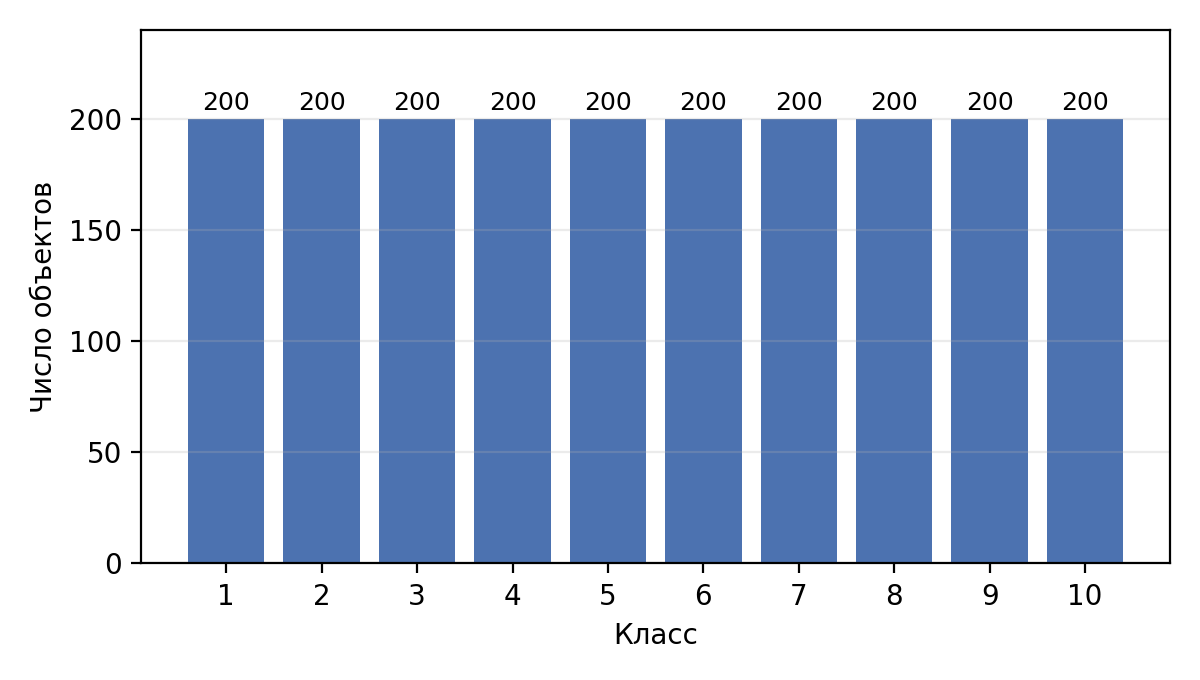
\includegraphics[width=0.6\textwidth]{images/class_dist.png}
    \caption{Распределение объектов по классам}
    \label{fig:classes}
\end{figure}

\begin{figure}[ht]
    \centering
    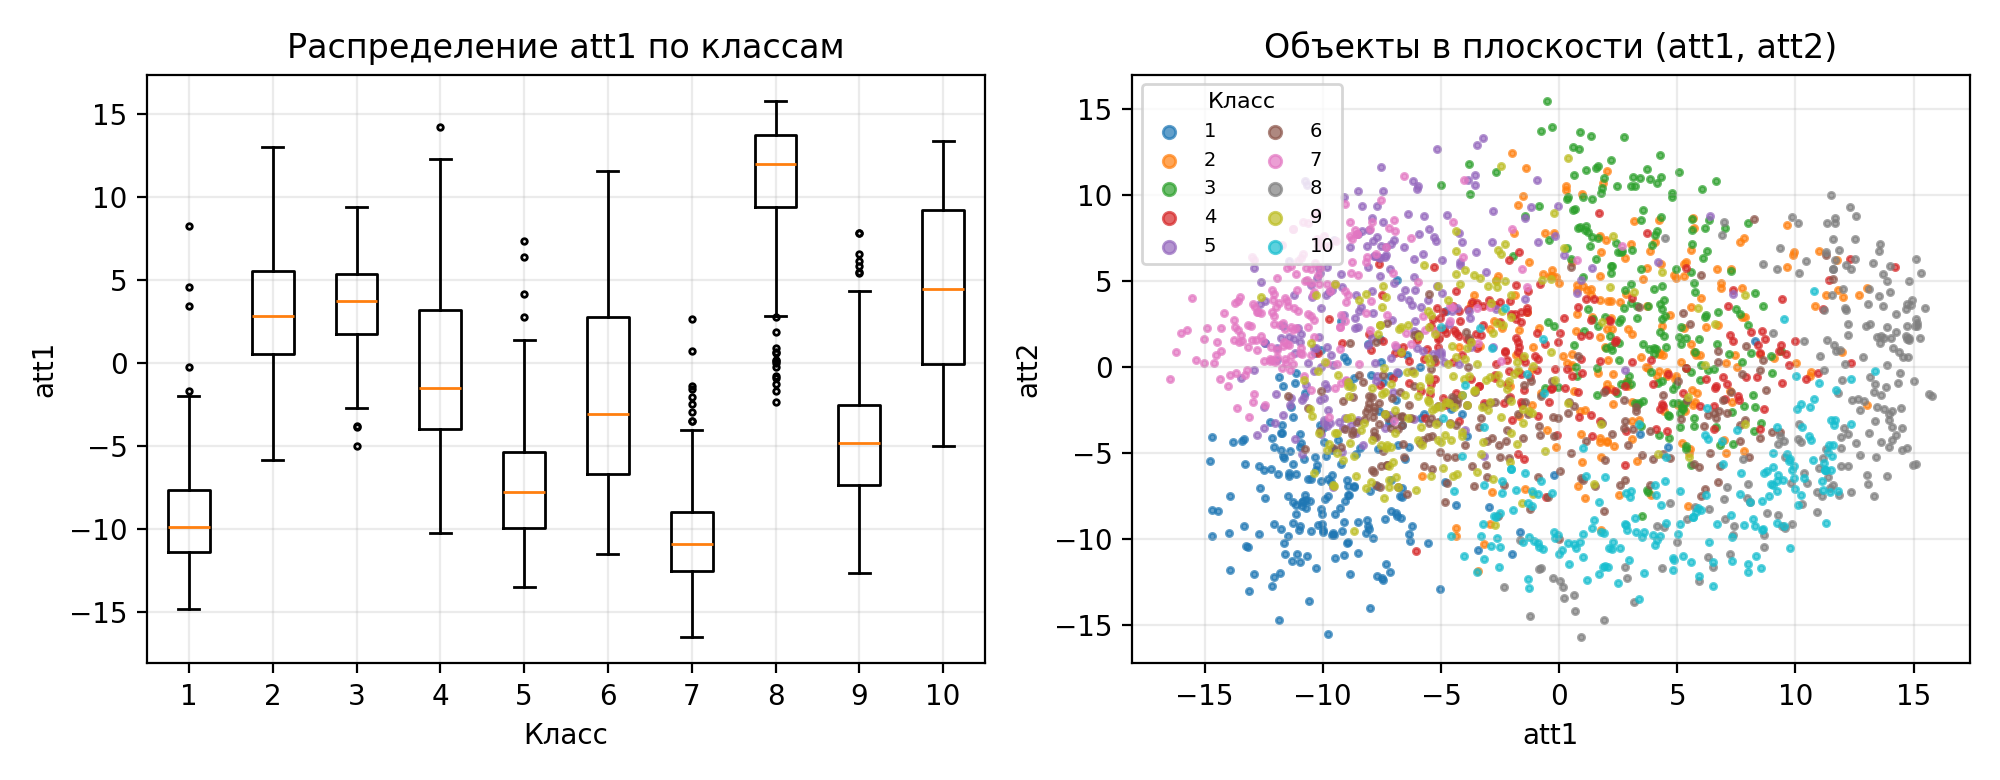
\includegraphics[width=\textwidth]{images/features.png}
    \caption{Признак \texttt{att1} по классам и объекты в плоскости (\texttt{att1}, \texttt{att2})}
    \label{fig:features}
\end{figure}

\section{Краткие теоретические сведения}
Для мини-пакета $X$ полносвязный слой записывается как $Z = XW + b$, $H = \varphi(Z)$. Без нелинейной активации $\varphi$ композиция слоёв эквивалентна одному линейному преобразованию, поэтому задача XOR не решается одним линейным нейроном. Для сети с одним скрытым слоем и ReLU прямой проход и функция потерь имеют вид
\begin{gather*}
Z^1 = XW^1 + b^1,\quad H = \mathrm{ReLU}(Z^1),\quad Z^2 = HW^2 + b^2,\quad P = \mathrm{softmax}(Z^2),\\
L = -\frac1m \sum_{i} \ln P_{i,y_i} + \frac{\lambda}{2}\left(\|W^1\|^2 + \|W^2\|^2\right).
\end{gather*}
Обратное распространение применяет правило цепочки справа налево. Для связки Softmax и кросс-энтропии $dZ^2 = (P-Y)/m$, далее
\begin{gather*}
dW^2 = H^{\top} dZ^2 + \lambda W^2,\quad db^2 = \sum dZ^2,\quad dH = dZ^2 (W^2)^{\top},\\
dZ^1 = dH \odot \mathbf 1[Z^1>0],\quad dW^1 = X^{\top} dZ^1 + \lambda W^1,\quad db^1 = \sum dZ^1.
\end{gather*}
На прямом проходе сохраняются $X$, $Z^1$, $H$ и $P$. Градиент проверяется центральной конечной разностью $g_{num} \approx [L(\theta+\varepsilon) - L(\theta-\varepsilon)]/(2\varepsilon)$. Оптимизаторы: SGD --- $\theta \leftarrow \theta - \eta g$; Momentum --- $v \leftarrow \beta v + g$, $\theta \leftarrow \theta - \eta v$; Adam использует экспоненциальные средние градиента и его квадрата. L2-регуляризация ограничивает рост весов, Dropout зануляет часть активаций только в режиме обучения, ранняя остановка возвращает параметры с лучшей validation loss.

\section{Ход работы и результаты}

\subsection{Линейный baseline}
\texttt{LogisticRegression} обучена заново на Train текущего разбиения с той же стандартизацией, что и у MLP. На validation получены \textbf{Accuracy = 0.9325} и \textbf{macro-F1 = 0.9327}. Это согласуется с результатами лабораторной №1 (CV macro-F1 = 0.9443).

\textit{Гипотеза:} нелинейная модель улучшит качество, так как классы частично пересекаются (рисунок~\ref{fig:features}) и линейная граница не может их полностью разделить; ограничивающий фактор --- небольшой объём Train.

\subsection{Ручной BackProp, gradient check и XOR}
В NumPy реализована сеть с одним скрытым слоем: He-инициализация $W^1$, нулевые смещения, устойчивый Softmax (сдвиг на максимальный логит), функции прямого прохода, кросс-энтропии и обратного прохода. Ключевой фрагмент обратного прохода приведён в листинге~\ref{lst:backward}.

\begin{listing}[ht]
\begin{minted}[breaklines, fontsize=\footnotesize]{python}
def backward_numpy(cache, y, parameters, l2=0.0):
    X, Z1, H, P = cache["X"], cache["Z1"], cache["H"], cache["P"]
    m = len(y)
    dZ2 = P.copy()
    dZ2[np.arange(m), y] -= 1.0
    dZ2 /= m                      # (P - Y) / m
    dW2 = H.T @ dZ2 + l2 * parameters["W2"]
    db2 = dZ2.sum(axis=0)
    dH = dZ2 @ parameters["W2"].T
    dZ1 = dH * (Z1 > 0)           # ReLU derivative
    dW1 = X.T @ dZ1 + l2 * parameters["W1"]
    db1 = dZ1.sum(axis=0)
    return {"W1": dW1, "b1": db1, "W2": dW2, "b2": db2}
\end{minted}
\caption{Обратный проход двухслойной сети (NumPy)}
\label{lst:backward}
\end{listing}

\newpage

\textbf{Проверка градиента.} Проверка выполнена на малой сети (64--5--10) и 8 объектах Train, $\varepsilon = 10^{-5}$; случайно выбрано 12 компонент градиента (таблица~\ref{tab:gradcheck}). Максимальная относительная ошибка равна $4.81\cdot10^{-10}$: аналитический и численный градиенты совпадают. Элемент $b^1[3]$ выбран случайно дважды, поэтому различных компонент 11.

\begin{table}[ht]
\centering
\small
\begin{tabular}{cccc}
\toprule
Параметр & Аналитический & Численный & Отн. ошибка \\
\midrule
$W^2[0,0]$ & 0.284840 & 0.284840 & $8.1\cdot10^{-12}$ \\
$W^1[8,1]$ & 0.016103 & 0.016103 & $4.6\cdot10^{-10}$ \\
$W^1[8,4]$ & 0.047225 & 0.047225 & $1.3\cdot10^{-10}$ \\
$b^2[3]$ & 0.014238 & 0.014238 & $4.8\cdot10^{-10}$ \\
$b^1[3]$ & 0.018261 & 0.018261 & $2.7\cdot10^{-10}$ \\
$b^2[8]$ & 0.047566 & 0.047566 & $2.4\cdot10^{-11}$ \\
$b^1[0]$ & 0.106404 & 0.106404 & $8.8\cdot10^{-11}$ \\
$b^2[5]$ & 0.011965 & 0.011965 & $1.2\cdot10^{-10}$ \\
$b^1[1]$ & $-0.129908$ & $-0.129908$ & $3.5\cdot10^{-11}$ \\
$b^1[4]$ & 0.030470 & 0.030470 & $1.5\cdot10^{-10}$ \\
$b^1[3]$ & 0.018261 & 0.018261 & $2.7\cdot10^{-10}$ \\
$W^2[1,0]$ & 0.100170 & 0.100170 & $3.8\cdot10^{-11}$ \\
\bottomrule
\end{tabular}
\caption{Сравнение аналитических и численных градиентов}
\label{tab:gradcheck}
\end{table}

\textbf{XOR.} Сеть 2--8--2 обучалась полным градиентным спуском ($\eta = 0.10$, L2 $=10^{-4}$, 3000 эпох). Функция потерь снизилась до 0.0064 (рисунок~\ref{fig:xor}), все четыре объекта классифицированы верно (таблица~\ref{tab:xor}). Одной прямой точки XOR не разделить, но скрытый слой с ReLU строит новые признаки, в пространстве которых классы линейно разделимы; без нелинейности композиция слоёв осталась бы линейной моделью.

\begin{figure}[ht]
    \centering
    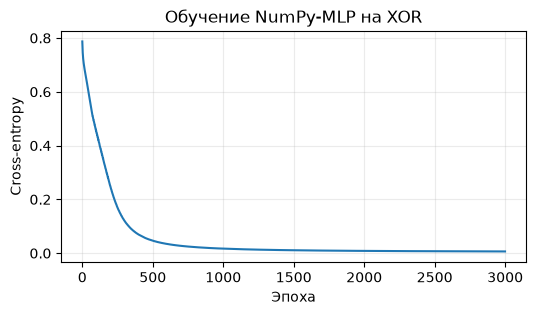
\includegraphics[width=0.7\textwidth]{images/xor.png}
    \caption{Функция потерь NumPy-MLP при обучении на XOR}
    \label{fig:xor}
\end{figure}

\begin{table}[ht]
\centering
\begin{tabular}{cccc}
\toprule
$x_1$ & $x_2$ & $P(y=1)$ & Предсказание \\
\midrule
0 & 0 & 0.010 & 0 \\
0 & 1 & 0.998 & 1 \\
1 & 0 & 0.999 & 1 \\
1 & 1 & 0.001 & 0 \\
\bottomrule
\end{tabular}
\caption{Результат NumPy-сети на XOR}
\label{tab:xor}
\end{table}

\subsection{MLP в PyTorch}
Архитектура: \texttt{Linear(64, 64)} $\to$ \texttt{ReLU} $\to$ \texttt{Dropout(p)} $\to$ \texttt{Linear(64, 10)}. Скрытый слой инициализируется по He, выходной --- по Xavier, смещения нулевые. Сеть возвращает логиты, поэтому \texttt{CrossEntropyLoss} получает их напрямую. Данные подаются через \texttt{TensorDataset} и \texttt{DataLoader} (batch 64 на обучении, 256 на оценке). Максимум 120 эпох, ранняя остановка с терпением 15 эпох по validation loss, по окончании восстанавливаются лучшие веса. Оценивание выполняется в режиме \texttt{model.eval()} под \texttt{torch.no\_grad()} (листинг~\ref{lst:train}).

\begin{listing}[ht]
\Needspace{18\baselineskip}
\begin{minted}[breaklines, fontsize=\footnotesize]{python}
model.train()                    # Dropout is active only in training
for X_batch, y_batch in train_loader:
    optimizer.zero_grad()        # do not accumulate old gradients
    logits = model(X_batch.to(DEVICE))
    loss = criterion(logits, y_batch.to(DEVICE))   # logits, not softmax
    loss.backward()
    optimizer.step()
val_metrics, _, _, _ = evaluate_model(model, val_loader)  # eval + no_grad
if val_metrics["loss"] < best_val_loss - 1e-5:
    best_val_loss = val_metrics["loss"]
    best_state = copy.deepcopy(model.state_dict())
    epochs_without_improvement = 0
else:
    epochs_without_improvement += 1
\end{minted}
\caption{Эпоха обучения с ранней остановкой}
\label{lst:train}
\end{listing}

Начальная конфигурация: Adam ($\eta=10^{-3}$), 64 скрытых нейрона, без регуляризации; обучение остановилось на 96-й эпохе. На рисунке~\ref{fig:curves} Train loss снижается почти до нуля, а Validation loss выходит на плато около 0.17 --- признак умеренного переобучения; validation macro-F1 стабилизируется около 0.957. Сравнение с baseline на validation приведено в таблице~\ref{tab:mlpval}: MLP превосходит логистическую регрессию по macro-F1 на 0.0246, гипотеза о пользе нелинейности подтверждается.

\begin{figure}[ht]
    \centering
    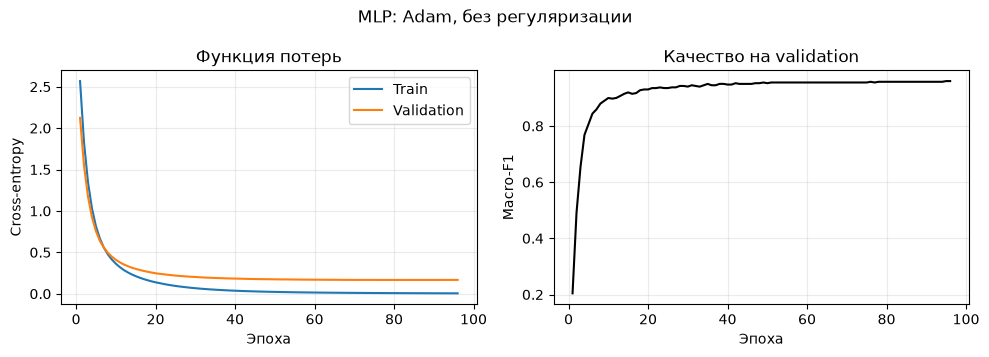
\includegraphics[width=\textwidth]{images/curves.png}
    \caption{Кривые обучения MLP (Adam, без регуляризации)}
    \label{fig:curves}
\end{figure}

\begin{table}[ht]
\centering
\small
\begin{tabular}{lcccc}
\toprule
Модель & Accuracy & macro-F1 & Cross-entropy & ROC-AUC \\
\midrule
LogisticRegression & 0.9325 & 0.9327 & --- & --- \\
MLP (Adam) & 0.9575 & 0.9573 & 0.1665 & 0.9980 \\
\bottomrule
\end{tabular}
\caption{Validation-метрики начальной MLP и baseline}
\label{tab:mlpval}
\end{table}

\subsection{Сравнение оптимизаторов}
SGD, Momentum и Adam сравнивались при одинаковых архитектуре, seed, разбиении и правиле остановки. Learning rate заданы заранее разных масштабов (таблица~\ref{tab:opt}): для Adam --- стандартный $10^{-3}$, так как его шаг нормируется по градиенту; для SGD --- 0.03; для Momentum ($\beta=0.9$) --- 0.02, поскольку инерция увеличивает эффективный шаг.

\begin{table}[ht]
\centering
\begin{tabular}{lcccc}
\toprule
Оптимизатор & $\eta$ & Эпох & best val loss & Val macro-F1 \\
\midrule
Adam & 0.001 & 96 & 0.1665 & 0.9573 \\
Momentum & 0.020 & 43 & 0.1823 & 0.9525 \\
SGD & 0.030 & 120 & 0.1830 & 0.9474 \\
\bottomrule
\end{tabular}
\caption{Сравнение оптимизаторов на validation}
\label{tab:opt}
\end{table}

Лучший результат у Adam (macro-F1 = 0.9573), он выбран для дальнейших экспериментов. Momentum остановился на 43-й эпохе, SGD дошёл до предела в 120 эпох без срабатывания ранней остановки. Разница между Adam и SGD по macro-F1 составляет около 0.01; сравнение проведено на одном seed.

\subsection{Сравнение Dropout и L2-регуляризации}
Для Adam ($\eta=10^{-3}$) сравнивались три режима; в каждом менялся только один механизм регуляризации (таблица~\ref{tab:reg}).

\begin{table}[ht]
\centering
\small
\begin{tabular}{lccccc}
\toprule
Режим & Dropout & weight\_decay & Эпох & val\_loss & Val macro-F1 \\
\midrule
Dropout & 0.25 & 0 & 109 & 0.1385 & 0.9600 \\
L2 & 0 & $10^{-4}$ & 113 & 0.1645 & 0.9598 \\
Без регуляризации & 0 & 0 & 96 & 0.1665 & 0.9573 \\
\bottomrule
\end{tabular}
\caption{Сравнение режимов регуляризации на validation}
\label{tab:reg}
\end{table}

Dropout дал наименьшую val loss (0.1385 против 0.1665 без регуляризации) и наибольший macro-F1 (0.9600); обучение до ранней остановки продолжалось дольше (109 эпох против 96), то есть переобучение наступает медленнее. L2 с $\lambda=10^{-4}$ почти не изменил результат (0.9598 против 0.9573). Различия macro-F1 между режимами малы (не более 0.0027 при 400 объектах в Validation). По правилу выбора (максимум validation macro-F1) выбрана конфигурация: \textbf{Adam, $\eta=10^{-3}$, 64 скрытых нейрона, Dropout 0.25, без weight decay}; число эпох для финального обучения --- 94 (эпоха с минимальной val loss выбранного запуска).

\subsection{Финальный test}
Схема preprocessing заново обучена на Train+Validation (1600 объектов), выбранная MLP обучена 94 эпохи, baseline переобучен на тех же данных. Test использован один раз. MLP превзошла логистическую регрессию и по Accuracy, и по macro-F1 (таблица~\ref{tab:test}); cross-entropy MLP на test равна 0.0859. Лучшая линейная модель ЛР №1 имела на test macro-F1 = 0.9675, у MLP --- 0.9824. Отчёт по классам --- в таблице~\ref{tab:report}, нормированная confusion matrix --- на рисунке~\ref{fig:cm}.

\begin{table}[ht]
\centering
\begin{tabular}{lccccc}
\toprule
Модель & Accuracy & Precision & Recall & F1-macro & ROC-AUC \\
\midrule
LogisticRegression & 0.9650 & --- & --- & 0.9649 & --- \\
MLP & 0.9825 & 0.9831 & 0.9825 & 0.9824 & 0.9989 \\
\bottomrule
\end{tabular}
\caption{Результаты на тестовой выборке}
\label{tab:test}
\end{table}

\begin{table}[ht]
\centering
\begin{tabular}{lcccc}
\toprule
Класс & Precision & Recall & F1-score & Support \\
\midrule
1 & 0.98 & 1.00 & 0.99 & 40 \\
2 & 0.95 & 1.00 & 0.98 & 40 \\
3 & 1.00 & 1.00 & 1.00 & 40 \\
4 & 1.00 & 0.90 & 0.95 & 40 \\
5 & 1.00 & 0.97 & 0.99 & 40 \\
6 & 0.95 & 1.00 & 0.98 & 40 \\
7 & 1.00 & 1.00 & 1.00 & 40 \\
8 & 0.98 & 1.00 & 0.99 & 40 \\
9 & 1.00 & 0.97 & 0.99 & 40 \\
10 & 0.97 & 0.97 & 0.97 & 40 \\
\midrule
\textbf{Accuracy} & \multicolumn{3}{c}{0.98} & 400 \\
\textbf{Macro avg} & 0.98 & 0.98 & 0.98 & 400 \\
\textbf{Weighted avg} & 0.98 & 0.98 & 0.98 & 400 \\
\bottomrule
\end{tabular}
\caption{Отчёт о классификации (MLP, test)}
\label{tab:report}
\end{table}

\begin{figure}[ht]
    \centering
    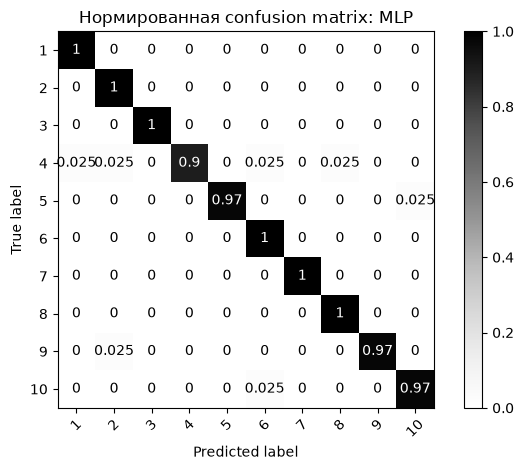
\includegraphics[width=0.6\textwidth]{images/cm.png}
    \caption{Нормированная матрица ошибок (Confusion Matrix) для MLP}
    \label{fig:cm}
\end{figure}

Слабее всего распознаётся класс 4 (recall = 0.90, 4 ошибки из 40); по одной ошибке допущено в классах 5, 9 и 10.

\subsection{Анализ ошибок}
Из 400 тестовых объектов ошибочно классифицированы 7 (таблица~\ref{tab:err}); столбец Idx --- позиция объекта в тестовой выборке. Для таблицы признаки выбраны по позициям \texttt{test\_index} (в ноутбуке строки \texttt{raw\_errors} идут в порядке возрастания индекса, а таблица ошибок отсортирована по уверенности, поэтому признаки выровнены заново).

\begin{table}[ht]
\centering
\begin{tabular}{cccccccc}
\toprule
Idx & true & pred & conf & att1 & att2 & att4 & att7 \\
\midrule
385 & 5 & 10 & 0.979 & $-3.19$ & $-5.17$ & 7.90 & $-3.15$ \\
231 & 4 & 1 & 0.969 & $-6.04$ & $-10.68$ & 6.01 & $-0.88$ \\
303 & 4 & 2 & 0.897 & 5.36 & 5.74 & 9.23 & $-1.71$ \\
308 & 10 & 6 & 0.680 & 1.84 & $-11.61$ & 5.41 & $-2.42$ \\
369 & 4 & 8 & 0.679 & 14.23 & 5.82 & 2.31 & $-1.68$ \\
315 & 9 & 2 & 0.617 & 1.77 & $-3.32$ & 7.01 & $-3.32$ \\
370 & 4 & 6 & 0.333 & $-4.37$ & 4.43 & 7.71 & 8.81 \\
\bottomrule
\end{tabular}
\caption{Ошибки MLP на test (по убыванию уверенности)}
\label{tab:err}
\end{table}

Четыре из семи ошибок приходятся на класс 4 (объекты 231, 303, 369, 370), которые ушли в четыре разных класса (1, 2, 8, 6). \textbf{Возможные причины ошибок:}
\begin{enumerate}
    \item \textbf{Перекрытие классов.} Объект 303 ($\texttt{att1}=5.36$, $\texttt{att2}=5.74$) лежит в области рисунка~\ref{fig:features}, где перемешаны классы 2, 3 и 4; близки к ней и ошибки 4$\to$2 и 9$\to$2. Класс 4 имеет широкий разброс по \texttt{att1}, поэтому пересекается с несколькими соседями.
    \item \textbf{Нетипичные значения признаков.} У объекта 369 значение $\texttt{att1}=14.23$ --- выброс для класса 4 (рисунок~\ref{fig:features}, слева) и типичное значение для класса 8, в который он и отнесён. Объект 231 ($\texttt{att1}=-6.04$, $\texttt{att2}=-10.68$) лежит в области класса 1, в который он и отнесён с уверенностью 0.969.
    \item \textbf{Возможный шум в данных и ограничения модели.} Объекты 385 и 231 классифицированы неверно с очень высокой уверенностью (0.979 и 0.969). Это может указывать на нестандартно написанные или неоднозначные цифры, а также на ограниченность модели с одним скрытым слоем, обученной на 1600 объектах.
\end{enumerate}

\section*{Выводы}
\begin{enumerate}
    \item Линейный baseline (\texttt{Logistic\-Regression}) показал на validation Accuracy = 0.9325 и macro-F1 = 0.9327, на test после переобучения на Train+Validation --- 0.9650 и 0.9649.
    \item Ручной BackProp реализован корректно: максимальная относительная ошибка по 12 проверенным компонентам градиента равна $4.81\cdot10^{-10}$. Сеть 2--8--2 решила XOR (loss 0.0064 за 3000 эпох, 4 из 4 объектов верно), что показывает роль скрытого слоя и нелинейности.
    \item Начальная MLP (64 нейрона, Adam, $\eta=10^{-3}$) на validation достигла macro-F1 = 0.9573 против 0.9327 у baseline, ROC-AUC = 0.9980; на кривых видно умеренное переобучение (Train loss $\to$ 0, Validation loss около 0.17).
    \item Среди оптимизаторов лучшим оказался Adam (macro-F1 = 0.9573), затем Momentum (0.9525) и SGD (0.9474); сравнение проведено на одном seed.
    \item Лучший режим регуляризации --- Dropout 0.25 (val macro-F1 = 0.9600, val loss = 0.1385 против 0.1665 без регуляризации); L2 с $\lambda=10^{-4}$ почти не повлиял (0.9598).
    \item На test выбранная MLP показала Accuracy = 0.9825, macro-F1 = 0.9824, ROC-AUC = 0.9989 против 0.9650 и 0.9649 у логистической регрессии; лучшая линейная модель ЛР №1 дала macro-F1 = 0.9675.
    \item Ошибки (7 из 400) сосредоточены в классе 4 (recall = 0.90, 4 ошибки); возможные причины --- перекрытие классов, нетипичные значения признаков и возможный шум в данных.
    \item Протокол соблюдён: preprocessing обучался только на Train (затем на Train+Validation), конфигурация выбрана по validation, test использован один раз; оценка выполнялась в \texttt{model.eval()} под \texttt{torch.no\_grad()}, градиенты обнулялись перед каждым мини-пакетом.
\end{enumerate}

\end{document}